\documentclass{article}

\usepackage{times}

\usepackage[final,dvips]{graphicx} % more modern

\usepackage{subfigure} 

% For citations
\usepackage{natbib}

% For algorithms
\usepackage{algorithm}
\usepackage{algorithmic}


\usepackage{hyperref}


\newcommand{\theHalgorithm}{\arabic{algorithm}}


\usepackage[accepted]{icml2014} 
\usepackage[section]{placeins}

\begin{document} 

\twocolumn[
\icmltitle{Final Report for ECE514\\A Convolutional Neural Network for Cassava Leaf Disease Classification}


\icmlauthor{Diamantis Georgios}{gdiamantis@uth.gr}
\icmlauthor{Kravariti Danai}{Skravariti@uth.gr}
\icmlauthor{Koen Leonardo}{lkoen@uth.gr}


\icmlkeywords{boring formatting information, machine learning}

\vskip 0.3in
]

\begin{abstract} 
This work is inspired by Kaggle competition which was part of the Fine-Grained Visual Categorization
workshop at CVPR 2019 (Conference on Computer Vision and Pattern Recognition). Using a dataset of 21,367 labeled images collected during a survey in Uganda we tried to develop a neural network to classify between 5 diseases: Cassava Bacterial Blight (CBB), Cassava Brown Streak Disease (CBSD), Cassava Green Mottle (CGM) and Cassava Mosaic Disease (CMD).
\end{abstract} 


\section{Introduction}
Cassava is one of the most common
food crops grown in sub-Saharan Africa. The
major challenge is that cassava plants are vulnerable to a broad
range of diseases. Because the detection of these diseases by humans is tiresome, we need an automated process than can detect these diseases in time so that they can be treated.This work shows the techniques used to achieve an accuracy score of over 86\%\, with a very imbalanced dataset of 21,367 labeled images (heavily biased towards classes – CMD and CBSD).

\section{Overview of the Diseases} 

\subsection{Cassava Bacterial Blight}
\begin{figure}[!htb]
    \centering
    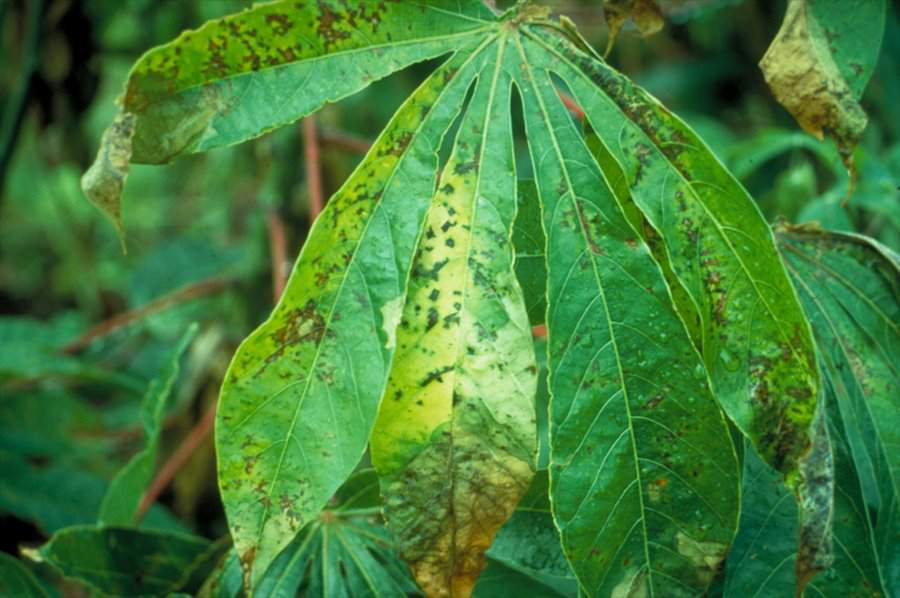
\includegraphics[width=0.4\textwidth]{cassavabb.png}
    \caption{Cassava Bacterial Blight}
    \label{CBB}
\end{figure}
Bacterial blight of cassava (Figure 1) is a serious problem in Central and South America. Symptoms include leaf spotting, wilting, die-back, gum exudation on young shoots, and vascular discoloration in mature stems and roots of susceptible cultivars\cite{J.C.Lozano}.


\subsection{Cassava Brown Streak Disease}

\begin{figure}[!htb]
    \centering
    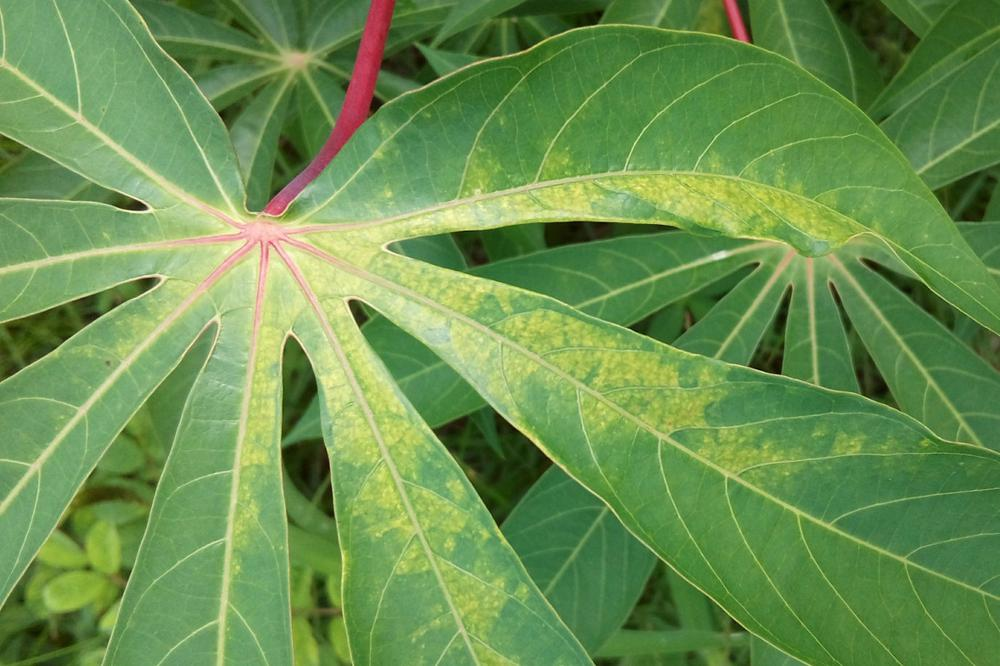
\includegraphics[width=0.4\textwidth]{cassava-brown-streak-disease-manioc-1.jpg}
    \caption{Cassava Brown Streak}
    \label{CBB}
\end{figure}
Cassava brown streak disease (CBSD) is
a devastating disease that causes loss of
cassava root (tuber) production and quality.
It can render susceptible varieties unusable
if cassava roots are left in the ground for
over nine months.Symptoms include: yellow patches mixed with green color (chlorosis), dark brown “streaks” and “spots” on stems, corky and yellow-brown necrotic spots on harvested roots.
\cite{fundament}



\subsection{Cassava Green Mottle}

\begin{figure}[!htb]
    \centering
    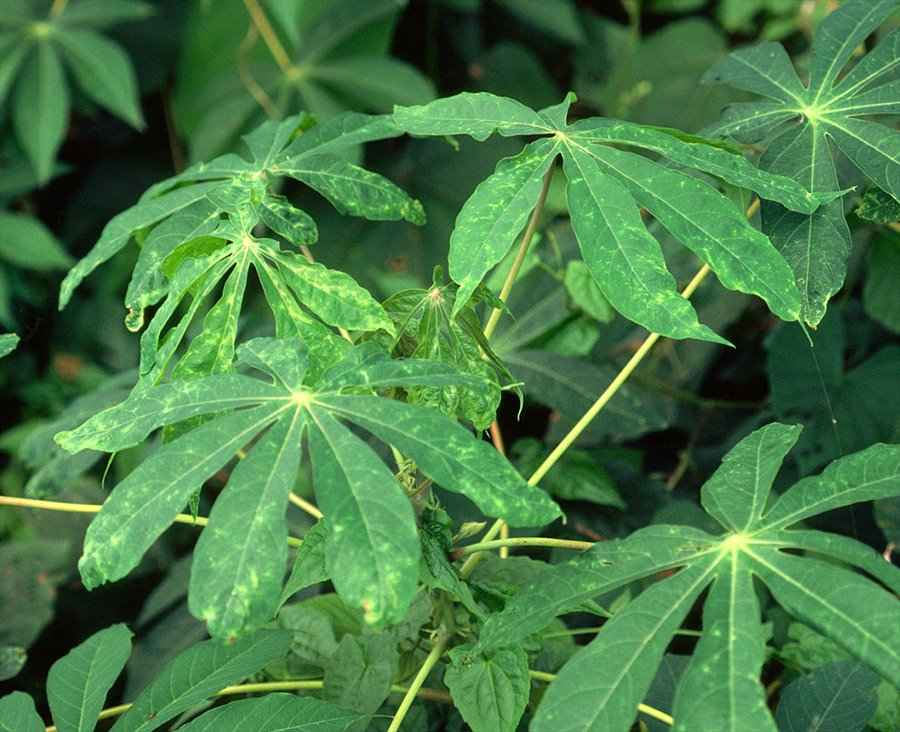
\includegraphics[width=0.4\textwidth]{cgmv.jpg}
    \caption{Cassava Green Mottle}
    \label{CBB}
\end{figure}

Leaves are puckered with distinct yellow spots, green patterns, and twisted margins. Usually, the shoots recover from symptoms and appear healthy. Occasionally, plants become severely stunted, edible roots are absent or, if present, they are small and woody when cooked.
\cite{fundament1}


\subsection{Cassava Mosaic Disease}
\begin{figure}[!htb]
    \centering
    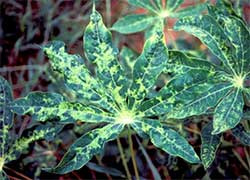
\includegraphics[width=0.4\textwidth]{image.jpeg}
    \caption{Cassava Mosaic Disease}
    \label{CBB}
\end{figure}


Cassava Mosaic Disease is the most severe and widespread. Cassava Mosaic Disease produces a variety of symptoms that include mosaic, mottling, misshapen and twisted leaflets, and an overall reduction in size of leaves and plants. Affected plants produce few or no tubers depending on the severity of the disease.



\cite{cmd}
\section{Model Architecture}

In order to classify these diseases we used a convolutional neural. The CNNs architecture contains three 2D Convolutional Layers followed by Batch Normalization and Max Pooling 2D Layers. At the end of the convolution the input vector is flattened with A Global Average Pooling 2D layer and then we have four additional Dense layers, one of which is the output layer. The first Conv2D layer has filter size of 32 and kernel size 5x5, the other two have filters 64 and 128 respectively and kernel size 3x3. All of them have padding equal to 'same' and the activation function is the ReLU function. All Max Pooling 2D layers have pool size 2x2. Finally there are four dense layers with 1024, 512, 256 and 5 neurons respectively and activation ReLU. The model is compiled with RMSProp optimizer.


\section{Methods}

The techniques used for addressing class imbalance were class weights, focal loss as a loss function and resampling minority class using SMOTE (Synthetic Minority Oversampling Technique). Focal loss and class weights led to very low accuracy scores. SMOTE on the other hand was proved to be very useful in terms of increasing accuracy. All the images were fed to the neural network as batches of 16 images. Also image augmentation techniques were used in order to avoid overfitting.

\begin{figure}
\centering
\begin{subfigure}{}
  \centering
  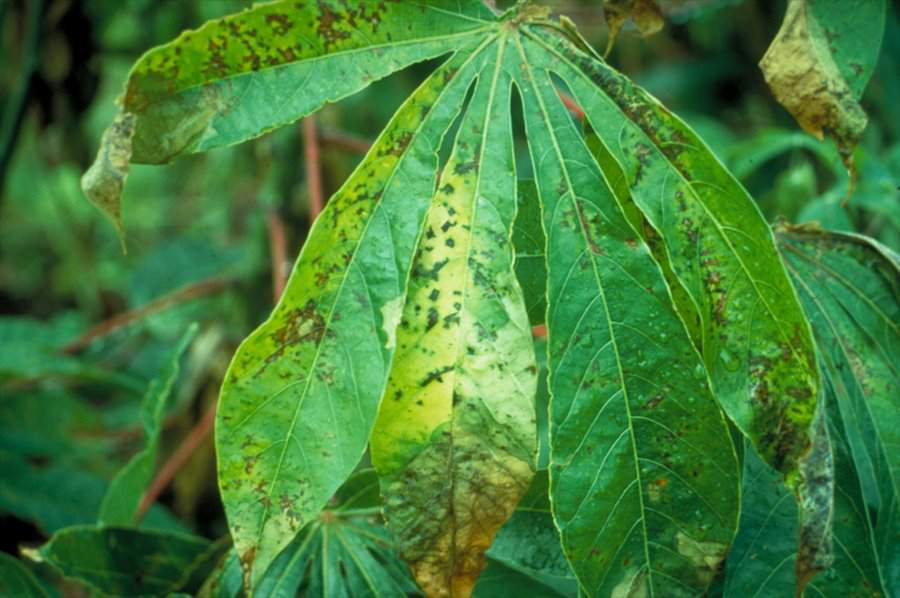
\includegraphics[width=.7\linewidth]{cassavabb.png}
  \caption{Before CLAHE}
  \label{fig:sub1}
\end{subfigure}%
\begin{subfigure}{}
  \centering
  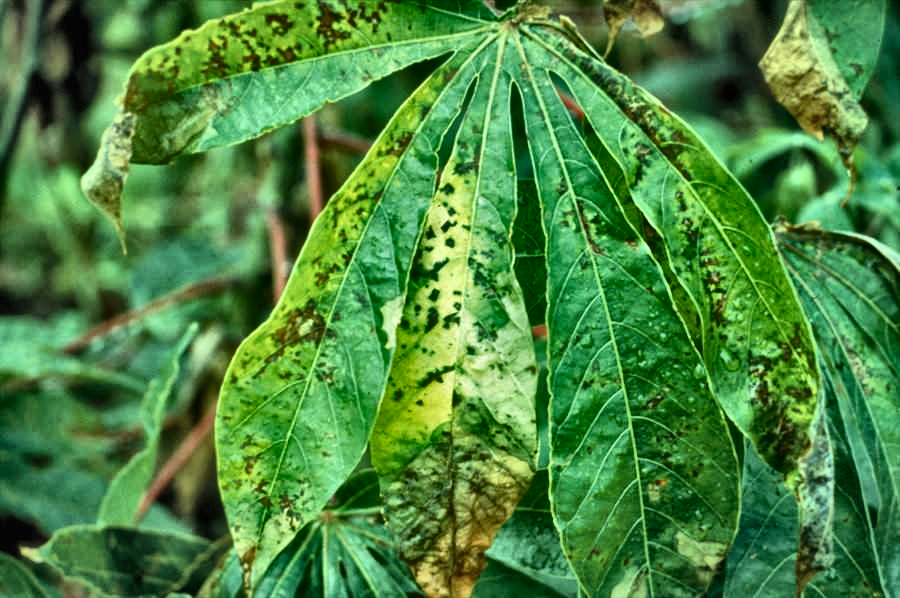
\includegraphics[width=.7\linewidth]{cassavabb_clahe.png}
  \caption{After CLAHE}
  \label{fig:sub2}
\end{subfigure}
\caption{Contrast Limited Adaptive Histogram Equalization (CLAHE)}
\label{fig:test}
\end{figure}

Adaptive histogram equalization (CLAHE) was used as an image preprocessing tool in order to increase the contrast of images (Figure 6). This can lead to better accuracy because high contrast images tend to help neural networks learn better.

\begin{figure}[!htb]
    \centering
    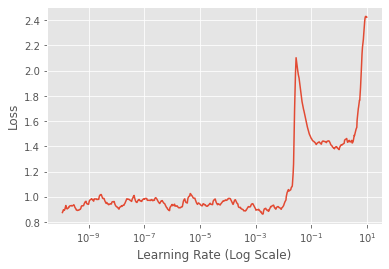
\includegraphics[width=0.4\textwidth]{index2.png}
    \caption{Learning rate finder results}
    \label{CBB}
\end{figure}

In order to find the optimal learning rate we used a learning rate finder algorithm (Figure 8) . Cyclical learning rate (Figure 9) techniques were also used in order to get the best out of the model.
\begin{figure}[!htb]
    \centering
    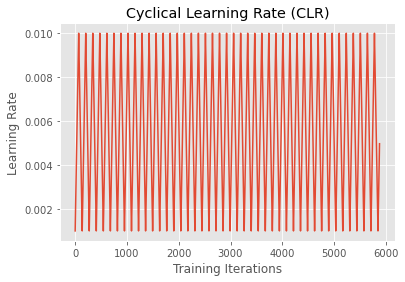
\includegraphics[width=0.4\textwidth]{index1.png}
    \caption{Cyclical learning rate}
    \label{CBB}
\end{figure}

\begin{figure}[!htb]
    \centering
    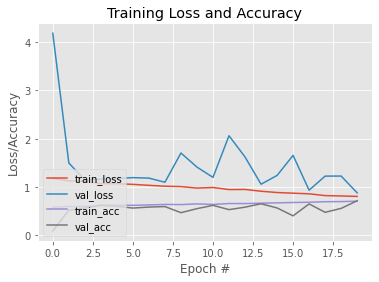
\includegraphics[width=0.4\textwidth]{index.png}
    \caption{Final accuracy results}
    \label{CBB}
\end{figure}

\section{Discussion}
This paper shows that image recognition can be very powerful tool for solving real life problems such as classifying the Cassava Diseases. The accuracy of this model can be further increased using a bigger dataset (more images) and tweaking it's hyperparameters.

\bibliography{example_paper}
\bibliographystyle{icml2014}

\end{document} 
